\documentclass[nobib]{tufte-handout}

%\\geometry{showframe}% for debugging purposes -- displays the margins

\newcommand{\bra}[1]{\left(#1\right)}
\usepackage{amssymb}
\usepackage{hyperref}
\usepackage[activate={true,nocompatibility},final,tracking=true,kerning=true,spacing=true,factor=1100,stretch=10,shrink=10]{microtype}
\usepackage{color}

% Fixes captions and images being cut off
\usepackage{marginfix}
\usepackage{array}
\usepackage{tikz}
\usepackage{amsmath,amsthm}
\usetikzlibrary{shapes}
\usetikzlibrary{positioning}
\usepackage{listings}
\usepackage{caption}
\DeclareCaptionFont{white}{\color{white}}
\DeclareCaptionFormat{listing}{\colorbox{gray}{\parbox{\textwidth}{#1#2#3}}}
\captionsetup[lstlisting]{format=listing,labelfont=white,textfont=white}

% Set up the images/graphics package
\usepackage{graphicx}
\setkeys{Gin}{width=\linewidth,totalheight=\textheight,keepaspectratio}
\graphicspath{{.}}

\title{Notes for ECE 369 - Discrete Mathematics for Computer Engineering}
\author[Ezekiel Ulrich]{Ezekiel Ulrich}
\date{\today}  % if the \date{} command is left out, the current date will be used

% The following package makes prettier tables.  We're all about the bling!
\usepackage{booktabs}

% The units package provides nice, non-stacked fractions and better spacing
% for units.
\usepackage{units}

% The fancyvrb package lets us customize the formatting of verbatim
% environments.  We use a slightly smaller font.
\usepackage{fancyvrb}
\fvset{fontsize=\normalsize}

% Small sections of multiple columns
\usepackage{multicol}

% For finite state machines 
\usetikzlibrary{automata} % Import library for drawing automata
\usetikzlibrary{positioning} % ...positioning nodes
\usetikzlibrary{arrows} % ...customizing arrows
\tikzset{node distance=2.5cm, % Minimum distance between two nodes. Change if necessary.
    every state/.style={ % Sets the properties for each state
    semithick,
    fill=gray!10},
    initial text={}, % No label on start arrow
    double distance=2pt, % Adjust appearance of accept states
    every edge/.style={ % Sets the properties for each transition
    draw,
    ->,>=stealth', % Makes edges directed with bold arrowheads
    auto,
    semithick}}
\let\epsilon\varepsilon

% These commands are used to pretty-print LaTeX commands
\newcommand{\doccmd}[1]{\texttt{\textbackslash#1}}% command name -- adds backslash automatically
\newcommand{\docopt}[1]{\ensuremath{\langle}\textrm{\textit{#1}}\ensuremath{\rangle}}% optional command argument
\newcommand{\docarg}[1]{\textrm{\textit{#1}}}% (required) command argument
\newenvironment{docspec}{\begin{quote}\noindent}{\end{quote}}% command specification environment
\newcommand{\docenv}[1]{\textsf{#1}}% environment name
\newcommand{\docpkg}[1]{\texttt{#1}}% package name
\newcommand{\doccls}[1]{\texttt{#1}}% document class name
\newcommand{\docclsopt}[1]{\texttt{#1}}% document class option name

% Define a custom command for definitions and biconditional
\newcommand{\defn}[2]{\noindent\textbf{#1}:\ #2}
\let\biconditional\leftrightarrow

\begin{document}

\maketitle

\begin{abstract}
These are lecture notes for fall 2023 ECE 36900 at Purdue. Modify, use, and distribute as you please.
\end{abstract}

\tableofcontents

\section{Course Introduction}

This course introduces discrete mathematical structures and 
finite-state machines. Students will learn how to use logical 
and mathematical formalisms to formulate and solve problems in 
computer engineering. Topics include formal logic, proof techniques, 
recurrence relations, sets, combinatorics, relations, functions, 
algebraic structures, and finite-state machines. For more information,
see the syllabus. 

\pagebreak 

\section{Equations}

\begin{enumerate}
    \item De Morgan's Theorem: 
    
    $\neg(P \wedge Q) \equiv \neg P \vee \neg Q$

    $\neg(P \vee Q) \equiv \neg P \wedge \neg Q$

    \item Modus ponens (mp)
    
    $p$

    $p \rightarrow q$

    $\therefore q$

    \item Modus tonens (mt)
    
    $p \rightarrow q$

    $\neg q$

    $\therefore \neg p$

    \item Predicate inference rules:
    \begin{table}[ht]
        \centering
        \begin{tabular}{|c|c|c|c|}
        \hline
        Name & Abrv. & Given & Can conclude\\
        \hline
        Existential generalization & eg & $P(a)$ & $(\exists x)P(x)$\\
        \hline
        Existential instantiation & ei & $(\exists x)P(x)$ & $P(a)$\\
        \hline
        Universal generalization & ug & $P(x)$ & $(\forall x)P(x)$\\
        \hline
        Universal instantiation & ui & $(\forall x)P(x)$ & $P(a)$\\
        \hline
        \end{tabular}
    \end{table}

    \item Propositional equivalence rules: 
    \begin{table}[ht]
        \centering
        \begin{tabular}{|c|c|c|}
        \hline
        Expression & Equivalent to & Name - abbreviation\\
        \hline
        $p \lor q$ & $q \lor p$ & Commutative - comm\\
        $p \land q$ & $q \land p $ &\\
        \hline
        $(p \lor q) \lor r$ &$p \lor (q \lor r)$ & Associative - ass\\
        $(p \land q) \land r$ &$p \land (q \land r)$ &\\
        \hline
        $\neg(p \wedge q)$ & $\neg p \vee \neg q$ & De Morgan's Laws - De Morgan\\
        $\neg(p \vee q)$ & $\neg p \wedge \neg q$ &\\
        \hline
        $p \rightarrow q$ & $\neg p \lor q$ & Implication - imp \\
        \hline
        $p$ & $\neg (\neg p)$ & Double negation - dn \\
        \hline
        $p \biconditional q$ & $(p \rightarrow q) \land (q \rightarrow p)$ & Def'n of equivalence - equ\\
        \hline
        \end{tabular}
    \end{table}
    \item Propositional inference rules: 
    \begin{table}[ht]
        \centering
        \begin{tabular}{|c|c|c|}
        \hline
        From & Can derive & Name - abbreviation\\
        \hline
        $p, p \rightarrow q$ & $q$ & Modus ponens - mp\\
        $p \rightarrow q, \neg q$ & $\neg p$ & Modus tollens - mt\\
        \hline
        $p, q$ & $p \land q$ & Conjunction - con\\
        \hline
        $p \lor q, \neg p$ & $q$ & Disjunction - dis\\
        \hline
        $p \land q$ & $p, q$ & Simplification - sim\\
        \hline
        $p$ & $p \lor q$ & Addition - add\\
        \hline
        \end{tabular}
    \end{table}
\end{enumerate}

\pagebreak

\pagebreak 

\section{Propositional Logic}

We often wish that others would be more logical, tell the truth,
or shower. While studying formal logic cannot help with the latter
(in fact, studies have shown a negative correlation between
hygiene and studying formal logic) it is a useful way to 
define what the first two mean. In a formal logic model, we have two constructs:
\begin{itemize}
    \item \defn{Statements/propostion}{A statement or a proposition is a sentence that
    is either true or false.} Propositions are often represented 
    with letters of the alphabet. For example: "$q$: the more time
    you spend coding, the less time you have to buy deodorant."
    \item \defn{Logical connectives}{Used to connect statements.} For 
    example, "and" is a logical connective in English. It can be
    used to connect two statements, e.g. "the person next to me
    smells like dog \emph{and} looks like a dog" to obtain 
    a new statement with its own truth value. 
\end{itemize}

Here are common logical connectives in Boolean logic:
\begin{table}[h]
    \centering
    \begin{tabular}{lc}
    \toprule
    \textbf{Logical Connective} & \textbf{Symbol} \\
    \midrule
    Negation (NOT) & $\lnot$ or $'$ \\
    Conjunction (AND) & $\land$ \\
    Disjunction (OR) & $\lor$ \\
    Exclusive OR (XOR) & $\oplus$ \\
    Implication & $\rightarrow$ \\
    Biconditional & $\leftrightarrow$ \\
    \bottomrule
    \end{tabular}
    \caption{Logical Connectives in Boolean Logic}
    \label{tab:logical-connectives}
\end{table}

\defn{Truth table}{Defines how each of the
connectives operate on truth values. Every connective has one.}
For example, consider $\land$ AND:

\begin{table}[ht]
    \centering
    \begin{tabular}{|c c|c|}
    \hline
    $p$ & $q$ & $p \land q$ \\
    \hline
    T & T & T \\
    T & F & F \\
    F & T & F \\
    F & F & F \\
    \hline
    \end{tabular}
    \caption{Truth table for $\land$}
    \label{tab:truthtableand}
\end{table}
We see that $p$ AND $q$ is only true when $p$ is true and 
$q$ is true. Similarly, $p$ or $q$ is only true when $p$ is true or 
$q$ is true (or both). An important connective for 
discovering new truths is the implication $\rightarrow$, which basically
says "if the first letter is true, then so is the second".
Let $p$: "I live in Wiley" and $q$: "I have no AC". In English,
the statement $p \rightarrow q$ would be stated as "If I live in 
Wiley, then I have no AC". 

\begin{table}[ht]
    \centering
    \begin{tabular}{|c c|c|}
    \hline
    $p$ & $q$ & $p \rightarrow q$ \\
    \hline
    T & T & T \\
    T & F & F \\
    F & T & T \\
    F & F & T\\
    \hline
    \end{tabular}
    \caption{Truth table for $\rightarrow$}
    \label{tab:truthtableimp}
\end{table}
Table \ref{tab:truthtableimp} shows the truth table for $\rightarrow$.
It may not seem immediately clear why, for instance, 
if $p$ and $q$ are false, then $p \rightarrow q$ is true.
If we consider what this means in English, then all we know is 
that I don't live in Wiley. Perhaps I live in Tarkington and still
don't have AC, or perhaps I live in Honors and I do. In any case
the first letter isn't true, so "if the first letter is true
then so is the second" stands as true. If we have the statement 
$p \rightarrow q$, then we call $q$ a \emph{necessary condition}
for $p$. Conversely, $p$ is a \emph{sufficient condition} for $q$.

Say we have a statement such as 
$A \lor B \rightarrow C$.
This is ambiguous, since we can interpret 
it as either $(A \lor B) \rightarrow C$ 
or $A \lor (B \rightarrow C)$. The truth tables
will differ in each case, so it 
becomes necessary to specify in
what order we should apply logical
connectives. 

\begin{enumerate}
    \item Parentheses "()"
    \item Negation "$\neg$"
    \item AND "$\land$"
    \item OR "$\lor$"
    \item Implication "$\rightarrow$"
    \item Biconditional "$\biconditional$"
\end{enumerate}

\pagebreak 

\section{Rules and proofs}

With each additional variable in your truth table, the number
of choices grows exponentially. Specifically, if you have $n$ statement
letters, you would have $2^n$ choices for your truth table. 

\defn{Tautology}{A formula that is true in every model.} 
Example: I am president of the tautology club because 
I am president of the tautology club. 

\defn{Contradiction}{A formula that is false in every model}. Examples:
"it is raining and it is not raining", "I am sleeping and I am awake", 
"I am a good student and I attend IU". 

\marginnote{Interestingly, it is possible to prove any statement
in a system where a contradiction exists. This is known as the 
\emph{principle of explosion}. To see how it works, consider
the following example: 

\begin{enumerate}
    \item $p$: Donuts are good for you.
    \item $q$: Unicorns exist. 
\end{enumerate}

I'll now assume the contradictory statement "donuts are good for you
and donuts are not good for you".

\begin{align*}
    \neg p \land p &\quad \text{(Given)} \\
    p &\quad \text{(1, simplification)} \\
    p \lor q &\quad \text{(2, addition)}\\
    \neg p &\quad \text{(1, simplification)}\\
    \therefore q &\quad \text{(3, disjunction)}
\end{align*}

Ergo, unicorns exist. 

}

Confusion often arises when negating a sentence such as 
"the book is thick and boring". An natural inclination is to 
negate it thus: "the book is not thick and not boring".
However, consider the truth table for this:
$p$: "the book is thick", $q$: "the book is boring". 
\begin{table}[ht]
    \centering
    \begin{tabular}{|c c|c|c|c|}
    \hline
    $p$ & $q$ & $p \wedge q$ & $\neg(p \wedge q)$ & $\neg p \wedge \neg q$\\
    \hline
    T & T & T & F & F\\
    T & F & F & T & F\\
    F & T & F & T & F\\
    F & F & F & T & T\\
    \hline
    \end{tabular}
    \label{tab:demorganswrong}
\end{table}
We can see the last two rows are not identical, therefore
the negation of "the book is thick and boring" is not 
"the book is not thick and not boring". For $p$ to be 
false, either the book must not be thick \emph{or} the
book must not be boring. This is summarized by 
\defn{De Morgan's Theorem}{
    \[\neg(P \wedge Q) \equiv \neg P \vee \neg Q\]
    \[\neg(P \vee Q) \equiv \neg P \wedge \neg Q\]
}

We now have a sufficient understanding of truth tables and 
logical connectives to come up with some useful rules. First of these 
are 
\defn{Modus ponens (mp)}{
    \begin{align*}
        &p \\
        &p \rightarrow q \\
        &\therefore q \\
    \end{align*}
}

and

\defn{Modus tollens (mt)}{
    \begin{align*}
        &p \rightarrow q \\
        &\neg q \\
        &\therefore \neg p \\
    \end{align*}
}

Below are two tables for commonly used rules.

\begin{table}[ht]
    \centering
    \caption{Equivalence rules}
    \begin{tabular}{|c|c|c|}
    \hline
    Expression & Equivalent to & Name - abbreviation\\
    \hline
    $p \lor q$ & $q \lor p$ & Commutative - comm\\
    $p \land q$ & $q \land p $ &\\
    \hline
    $(p \lor q) \lor r$ &$p \lor (q \lor r)$ & Associative - ass\\
    $(p \land q) \land r$ &$p \land (q \land r)$ &\\
    \hline
    $\neg(p \wedge q)$ & $\neg p \vee \neg q$ & De Morgan's Laws - De Morgan\\
    $\neg(p \vee q)$ & $\neg p \wedge \neg q$ &\\
    \hline
    $p \rightarrow q$ & $\neg p \lor q$ & Implication - imp \\
    \hline
    $p$ & $\neg (\neg p)$ & Double negation - dn \\
    \hline
    $p \biconditional q$ & $(p \rightarrow q) \land (q \rightarrow p)$ & Def'n of equivalence - equ\\
    \hline
    \end{tabular}
    \label{tab:equivalencerules}
\end{table}

\begin{table}[ht]
    \centering
    \caption{Inference rules}
    \begin{tabular}{|c|c|c|}
    \hline
    From & Can derive & Name - abbreviation\\
    \hline
    $p, p \rightarrow q$ & $q$ & Modus ponens - mp\\
    $p \rightarrow q, \neg q$ & $\neg p$ & Modus tollens - mt\\
    \hline
    $p, q$ & $p \land q$ & Conjunction - con\\
    \hline
    $p \lor q, \neg p$ & $q$ & Disjunction - dis\\
    \hline
    $p \land q$ & $p, q$ & Simplification - sim\\
    \hline
    $p$ & $p \lor q$ & Addition - add\\
    \hline
    \end{tabular}
    \label{tab:inferencerules}
\end{table}

At this point, let us formally define an 

\defn{Argument}{An argument can be symbolized as 
\[P_1 \lor P_2 \lor P_3 \lor ... \lor P_n \rightarrow Q\] 
where $P_i$ is called a hypothesis and $Q$ is the conclusion.} If this statement
is a tautology, then the argument is \emph{valid}. 
There are multiple ways we could prove a given argument is a tautology.
For instance, we could create a truth table and brute force an answer.
However, with even four hypotheses this process is tedious, and with each additional hypothesis
it becomes exponentially harder. Therefore we instead often turn to the

\defn{Proof sequence}{a sequence of well-formed formulas 
in which each formula is either a premise or the result 
of applying a derivation rule to earlier well-formed formulas.} In practice this looks like
\begin{align*}
    P_1 \quad &\text{(hypothesis)}\\
    P_2 \quad &\text{(hypothesis)}\\
    P_3 \quad &\text{(hypothesis)}\\
    &\dots \\
    P_n \quad &\text{(hypothesis)}\\
    \text{(formula) }1 \quad &\text{(obtained from derivation rule)} \\
    \text{(formula) }2 \quad &\text{(obtained from derivation rule)} \\
    &\dots \\
    \text{(formula) } n \quad &\text{(obtained from derivation rule)} \\
    \therefore Q \\
\end{align*}

Let's use all this new information in a simple proof. 
\begin{align*}
    A \quad &\text{(hypothesis)}\\
    A \rightarrow B \quad &\text{(hypothesis)}\\
    B \rightarrow C \quad &\text{(hypothesis)}\\
    B \quad &\text{(1, 2, mp)}\\
    C \quad &\text{(4, 3, mp)}\\
    \hline
    \therefore C \notag
\end{align*}
If we wish to apply our knowledge of logic to the real world, 
some practice in translating natural language to formal logic 
is necessary. Let's test it with this statement: "If chicken is on
the menu, then don't order fish, but you should have either fish or salad.
So if chicken is on the menu, have salad." 
Let $C$: "Chicken is on the menu", $F$: "You order fish", and $S$: "You have salad".
We know that if chicken is on the menu you don't order fish, that you should have
either fish or salad, and we'd like to show that if chicken is on the menu 
you should have salad.
\begin{align*}
    C \quad &\text{(hypothesis)}\\
    C \rightarrow \neg F \quad &\text{(hypothesis)}\\
    F \lor S \quad &\text{(hypothesis)}\\
    \neg F \quad &\text{(1, 2, mp)}\\
    S \quad &\text{(3, 4, dis)}\\
    \hline
    \therefore S \notag
\end{align*}

\pagebreak 

\section{Predicate logic}
\defn{Predicate logic}{Capable of making statements about entire 
groups instead of individual letters. In predicate logic, 
propositions are expressed in terms of predicates, 
variables and quantifiers}, the latter of which propositional logic lacks. 

\defn{Quantifer}{How many objects have a certain property: "for every" or "for some".}

\defn{Predicate}{Property that a variable may have.}

\defn{Domain of interpretation}{Collection of objects from which the variable is taken.}

\defn{Universal quantifer}{"For all": $\forall$}. States that a certain property holds
for all objects in a domain. 

\defn{Existential quantifer}{"There exists": $\exists$}. States that a certain property holds
for at least one object in a domain. 

As an example of a predicate well-formed formula: $(\forall x)[(\exists y) x > y]$. We would read this statment as 
"for all $x$ there exists a $y$ such that $x > y$." At first glance it may seem 
obvious that this statement is true, but consider the domain. What if the domain is 
all natural numbers? Then we could let $x=1$ (or zero depending
or your definition of natural numbers) and there would be no corresponding
lesser $y$. We can see from this example that the truth value of 
a predicate logic formula depends on the domain as well as quantifiers and predicates. 

Just as with propositional logic, we often need to translate English statements
into predicate logic. Take the statement "every movie made by George Lucas is great".
We can rephrase this as "for any movie, if the movie is made by George Lucas, it is great".
We would write this formula as
\[(\forall x)(GL(x) \rightarrow Great(x))\]
(Author's note: no value judgement is associated with this
English statement).

Let's examine some rules in predicate logic. First, negation: 
\[\neg [\forall x A(x)] \biconditional (\exists)x \neg A(x)\]
Some rules from propositional logic still apply in predicate logic. Take 
modus ponens as an example:
\begin{align*}
    (\forall x)(\forall y)L(x,y) \rightarrow [(\exists x) H(x)] \quad &\text{(hypothesis)}\\
    \neg [(\exists x) H(x)] \quad &\text{(hypothesis)}\\
    \neg [(\forall x)(\forall y)L(x,y)] \quad &\text{(1, 2, mt)}\\
    (\exists x) (\exists y) \neg L(x,y) \quad &\text{(3, DM)}\\
    \hline
    \therefore (\exists x) (\exists y) \neg L(x,y) \notag
\end{align*}
Table \ref{tab:predinferencerules} holds predicate inference rules. 
\begin{table}[ht]
    \centering
    \caption{Predicate inference rules}
    \begin{tabular}{|c|c|c|c|}
    \hline
    Name & Abrv. & Given & Can conclude\\
    \hline
    Existential generalization & eg & $P(a)$ & $(\exists x)P(x)$\\
    \hline
    Existential instantiation & ei & $(\exists x)P(x)$ & $P(a)$\\
    \hline
    Universal generalization & ug & $P(x)$ & $(\forall x)P(x)$\\
    \hline
    Universal instantiation & ui & $(\forall x)P(x)$ & $P(a)$\\
    \hline
    \end{tabular}
    \label{tab:predinferencerules}
\end{table}
These rules hold given certain conditions. Namely:
\begin{enumerate}
    \item[(eg)] $x$ not in $P(a)$ 
    \item[(ei)] Must the be first rule that introduces $a$ 
    \item[(ug)] $P(x)$ not derived from a hypothesis
    with $x$ as a free variable, and $P(x)$ is not derived by ei from wff with $x$ as a free variable. 
    \item[(ui)] $a$ is a constant. 
\end{enumerate}
\marginnote{A \emph{free variable} is a variable not bound by a quantifer. For
example, in the formula 
\[(\forall x)(\forall y)P(x,y)\]
both $x$ and $y$ are bound by quantifers. Constrast this with the formula
\[(\exists x)(\forall y)q(x, y, z)\]
In this example, $z$ is a free variable, since it is not associated with 
any quantifiers.}
Let's see some of these rules in action by with a predicate logic proof.
Say we have the statement "every ECE student works harder
than somebody, and everyone who works harder than any other
person gets less sleep than that person. Maria is an 
ECE student. Ergo, Maria gets less sleep than someone. 
Let $E(x)$: "x is an ECE student", $W(x,y)$: "x works harder than y", 
$S(x,y)$: "x gets less sleep than y", and $m$: Maria. 
We want to prove $\exists a (S(m,a))$. 
\begin{align*}
    \forall x, E(x) \rightarrow (\exists y) (W(x,y)) \quad &\text{(hypothesis)}\\
    \forall x, \forall y (W(x,y) \rightarrow S(x,y)) \quad &\text{(hypothesis)}\\
    E(m) \quad &\text{(hypothesis)}\\
    \exists y (E(m) \rightarrow S(m,y)) \quad &\text{(1, ui)}\\
    E(m) \rightarrow W(m,a) \quad &\text{(4, ei)}\\
    \forall y (W(m,y) \rightarrow S(m,y)) \quad &\text{(3, ui)}\\
    %the above line doesn't make sense to me
    W(m,a) \rightarrow S(m,a) \quad &\text{(6, ui)}\\
    W(m,a) \quad &\text{(3,5 mp)}\\
    S(m,a) \quad &\text{(7,8, mp)}\\
    \exists a (S(m,a)) \quad &\text{(9, eg)}\\
    \hline
    \therefore \exists a (S(m,a)) \notag
\end{align*}
%I'm pretty sure this proof is wrong, I'll fix it later
\pagebreak 

\section{Proofs}
List of common proof techniques:
\begin{enumerate}
    \item Exhaustive proof: 
    In this kind of proof, the statement to be proved is 
    split into a finite number of cases or sets of equivalent 
    cases, and where each type of case is checked to see if 
    the proposition in question holds
    \item Refuting by counter-example: 
    If we have a universal statement such as 
    $\forall x (P(x) \rightarrow Q(x))$, we may
    show it to be false by finding a single $a$ 
    such that $\neg P(a)$. 
    \item Direct proof: 
    Trying to prove $p \rightarrow q$, start by 
    assuming $p$ and then show $q$. 
    \item Proof by contraposition: 
    The contrapositive of $p \rightarrow q$
    is $\neg q \rightarrow \neg p$. A statement 
    and its contrapositive are logically equivalent, so 
    if proving $p\rightarrow q$ is too difficult 
    we may try to prove $\neg q \rightarrow \neg p$ instead. 
    \item Proof by contradiction: 
    Suppose I have to prove $p \rightarrow q$. I can begin 
    by saying $p$ is true and $\neg q$ is true. If by a series of 
    steps I arrive a contradiction, then I may say $p$ implies $q$. 
    \item Proof by induction: employs a neat trick which 
    allows you to prove a statement about an arbitrary number 
    $n$ by first proving it is true when $n=1$ (or some other base case), 
    assuming it is true for $n=k$, and then showing it is true for $n=k+1$.
    The steps to prove $\forall n P(n)$ are:
    \begin{enumerate}
        \item Prove $P(1)$ (this is your \emph{base case}). 
        \item Assume for arbitrary $k \geq 1$, $P(k)$ (your \emph{inductive hypothesis}).
        \item Prove $P(k+1)$. 
    \end{enumerate}
\end{enumerate}
Below are some example proofs using each of these techniques. 
\begin{enumerate}
    \item \emph{Exhaustive proof (cases)}: say we wish to prove $|xy| = |x||y|$. 
    Let's split this into four cases:
    \begin{enumerate}
        \item Case 1: $x$ and $y$ positive.
        Then the absolute values are equal to the original
        numbers, and we have 
        \begin{align*}
            |x| &= x \\
            |y| &= y \\
            |xy| &= xy \\
            |x||y| &= xy \\
            \therefore |xy| &= |x||y|
        \end{align*}
        \item Case 2: $x$ and $y$ negative. 
        If $x$ and $y$ are both negative, then 
        $xy$ is positive. We thus have that 
        \begin{align*}
            |x||y| &= xy \\
            |xy| &= xy \\
            \therefore |xy| &= |x||y| 
        \end{align*}
        \item Case 3: $x$ negative and $y$ positive. 
        Now we have that $xy$ is negative. Still, though, 
        $|xy|$ will be positive (by def'n of ||), and so will 
        $|x|$ and $|y|$. So we again have that 
        \begin{align*}
            |xy| &= |x||y| 
        \end{align*}
        \item Case 4: $x$ positive and $y$ negative. 
        WLOG, case 3. 
    \end{enumerate}
    \begin{align*}
        \therefore |xy| &= |x||y| \qed
    \end{align*}
    \item \emph{Direct proof}: say we wish to prove the product of two even integers is even. 
    We first need to translate this English sentence to a mathematical 
    statement, which we can do in this case like so:
    \[x = 2a, a \in \mathbb{Z}, y = 2b, b \in \mathbb{Z}, \rightarrow x \times y = 2c, c \in \mathbb{Z}\]
    Our proof is below. 
    \begin{align*}
        x &= 2a, a \in \mathbb{Z} \\
        y &= 2b, b \in \mathbb{Z} \\
        z &= x \times y \\
        &= 2a\times 2b \\
        &= 2(2ab) \\
        &= 2c, c \in \mathbb{Z} \qed
    \end{align*}
    Since $c$ is an integer, $2c$ is even and the proof is complete. Try proving 
    the product of two odds is odd in a similar fashion. 
    \item \emph{Proof by contradiction}: say we wish to prove $\sqrt{2}$ is irrational. In a theme
    that will become common as we see more proofs by contradiction, 
    assume the opposite. That is, assume $\sqrt{2}$ is rational. By
    the definition of rational, we can then write 
    \[\sqrt{2} = \frac{a}{b}, a,b \in \mathbb{Z}\]
    Where $a$ and $b$ share no common factors. 
    We can then perform the following series of steps. 
    \begin{align*}
        \sqrt{2} &= \frac{a}{b} \\
        b\sqrt{2} &= a \\
        2b^2 &= a^2
    \end{align*}
    This means that $a^2$ is even. It can be easily shown 
    that if $a^2$ is even then $a$ is even. That means that 
    $a^2$ will actually be divisible by 4. We can rearrange to get
    \begin{align*}
        2b^2 &= 4c, c \in \mathbb{Z} \\
        b^2 &= 2c
    \end{align*}
    So $b$ is likewise even. But if both $a$ and $b$ are even, 
    then they share a common factor and our original supposition is false. 
    Ergo $\sqrt{2}$ is irrational. $\qed$. 
    \item \emph{Poof by induction}: say we wish to show 
    \[\sum_{i = 1}^{n} = \frac{n(n+1)}{2}\]
    Begin with the base case $n=1$. 
    \begin{align*}
        \sum_{i = 1}^{1} &= 1 \\
        &= \frac{1(1+1)}{2} \\
        &= \frac{n(n+1)}{2}
    \end{align*}
    Since we have shown the base case to be true, 
    we may now make our inductive hypothesis and assume that for
    arbitrary $k \geq 1$, 
    \begin{align*}
        \sum_{i = 1}^{k} &= \frac{k(k+1)}{2}
    \end{align*}
    Let us now show that the formula holds for $k + 1$. 
    \begin{align*}
        \sum_{i = 1}^{k + 1} &= \sum_{i = 1}^{k} + (k + 1)\\
        &= \frac{k(k+1)}{2} + (k + 1) \\
        &= \frac{k(k+1) + 2(k+1)}{2}\\
        &= \frac{k^2+3k+2}{2}\\
        &= \frac{(k + 1)(k + 2)}{2} \\
        &= \frac{(k + 1)((k+1) + 1)}{2} 
    \end{align*}
    And we are done $\qed$. 
\end{enumerate}
The form of induction we have just seen is the \emph{weak} form of 
induction. The \emph{strong} form of induction is the following.
\marginnote{The strong form is also known as the \emph{second principle of mathematical induction}}
To prove $\forall x, P(x)$, we still prove the base case ($P(n)$). 
Now, however, we assume for arbitrary $k \geq 1$ that $P(r)$ is 
true for $1 \leq r \leq k$ and try to prove $P(k+1)$.
Let's see this in action. Say we'd like to prove any postage 
greater than or equal to 8 cents can be created with a combination 
of 3 cent and 5 cent postage stamps. First, the base case. 8 can be 
created like so: $3+5 = 8$. Now let's assume for all $8 \leq r \leq k$, 
$P(r)$. Now the tricky part. To prove $P(k+1)$, notice that
\begin{align*}
    P(k+1) &= k+1 \\
    &= (k-2) + 3 \\
    &= (3a+5b) + 3 \\
    &= 3c + 5b \qed
\end{align*}
We had to rewrite $k+1$ as $k-2 + 3$ so we could 
use our assumption that $P(k-2)$ is true. 
\marginnote{We see that simply assuming $P(k)$
wouldn't be sufficient in this case, so there are proofs where we can 
use strong induction but not weak induction. Anything that can be proved
with weak induction can be proved with strong induction, since in 
strong induction we assume $P(k)$ in addition to $P(r)$ for all $r$ between 
$1$ and $k$. Hence, "strong".}
The astute among you will recognize that our proof is technically
imcomplete. We have assumed $P(k-2)$, but what if we wish to prove $P(9)$? 
This is not included in our inductive step, since we only assume $P(r)$ 
for $8\leq r \leq k$. We are in the domain of natural numbers (unless you
have somehow managed to find a postage stamp with negative or fractional value),
then there is no $r$ for which this is true. Therefore we also need to prove 
$P(9)$ and $P(10)$, which is pretty simple. 

Let's see a more advanced example 
of induction. Say you have a set of $n$ elements, and you want to create subsets of this set. 
You are interested in knowing how many subsets exist. After trying it out with 
$n=1,2,3$ you suspect the number of subsets that can exist is $2^n$, and you see
that this problem is a good candidate for induction. Your base case is 
$P(1) = 2 = 2^1$, so that's out of the way. Now assume $P(k)$. That is, for any 
set with $k < n$ elements, the number of subsets is $2^k$. You now need to show 
$P(k+1)$, which can be done by noticing that if we add an additional element to the set, 
then for every pre=existing group you can add the new element to get $2^k$ new groups, bringing your total 
number of subsets to $2^k+2^k=2\times2^k = 2^{k+1}$, and we are done.  

We've seen some examples of when induction is used well, but doing everything 
perfectly is tiring. Let's show something false: any group of horses are 
all the same color. Obviously the base case is true: a group of one horse 
is always the color of that horse. Assume $P(k)$, that any group of $k$ horses 
is monochromatic. Now we need to prove it for $k+1$. First, exclude one horse and 
look only at the other $k$ horses; all these are the same color, since $k$ horses 
always are the same color. Likewise, exclude some other horse (not identical to 
the one first removed) and look only at the other $k$ horses. By the same reasoning, 
these, too, must also be of the same color. Therefore, the first horse that 
was excluded is of the same color as the non-excluded horses, who in turn are 
of the same color as the other excluded horse. Hence, the first horse excluded, 
the non-excluded horses, and the last horse excluded are all of the same color, 
and we are done. What's the issue here? The issue is that in order to select two different 
horses, we need at least two different horses. However, our base case was with one horse. 
To use this logic we would need to show $P(2)$, for which our original argument is
obviously not true. 

\pagebreak 

\section{Proofs of correctness}

Say you are part of a team developing software for the NSA or NASA. 
A common requirement for the deliverable is to prove that it meets 
certain properties. You may be asked to show that your code 
will eventually return an answer (i.e. the algorithm terminates)
or that, \emph{if} an answer is returned, it will be correct. 
Correct in this sense means your program meets whatever specifications 
have been laid out. 

Broadly speaking, there are two properties that a program must 
satisfy. The first is 
\defn{safety}{the program will not violate any invariant that you write 
(think \texttt{assert} for C programs. If you always need to return 
a positive integer, for instance, and you can show that it always does, 
then you have satisfied safety)}. The second is 
\defn{liveness}{that your program is going to terminate}. This can be 
done by showing there are no infinite loops, for example. You may also specify
the amount of time in which your program is guarenteed to terminate. 
In the field, the longest possible time your program will take 
is known as Worst Case Execution Time (WCET).

In software development, as you are likely aware, your code is often checked 
using tests. This is one method of gaining evidence that the kernel of your 
program is correct. 
\marginnote{Note that "testing can prove the presence of errors 
but never their absence". We cannot show through testing that a program
will behave exactly as it should in all cases, unless the number of possible 
inputs is so small that it is possible to enumerate through them. Even though 
testing cannot prove the correctness of a program, it can still reveal issues
and build confidence that the code is correct. }
We may also prove that the code is correct, which is 
often more laborious. Unless you're developing software for safety-critical 
areas, you'll probably use testing more than formal proof. If you needed 
to unequivocally show that your program will do what it 
should under all circumstances of interest, you'll have to use formal 
logic techniques. 

To understand how we can apply logical rules to programming, imagine 
your algorithm as a function $P$ that takes in some input values $X$
and produces some output values $Y$. 
\[Y = P(X)\]
The predicate $Q(X)$ describes conditions that the input values 
will satisfy (e.g. $X > 0$, $X \in \mathbb{R}$, $X$ is a string under 127
characters). The predicate $R(X,Y)$ describes conditions that the output must satisfy
for a given input (e.g. $Y = \sqrt{X}$, $Y$ gives the prime factorization of $X$, 
$Y$ capitalizes $X$). We say a program is correct if the implication
\[\forall X[Q(X) \rightarrow R(X,P(X))]\]
is valid. That is, whenever $Q(X)$ is true of the inputs, $R(X,Y)$ should 
be true of the outputs. The notation changes when dealing with 
program correctness: here's the more common way to write the above implication:
\[\{Q\}P\{R\}\]
The terminology here is that $Q$ is a \emph{precondition} for program $P$, 
and $R$ is the \emph{postcondition}.
\marginnote{
$\{Q\}P\{R\}$ is called a \emph{Hoare triple} and gives 
before and after conditions for a program fragment. For instance, 
precondition: $Q(x)$, program: $Y = P(x)$, postcondition: $R(x,y)$
is a Hoare triple that means 
\begin{align*}
    (\forall X) Q(X) &\rightarrow R(X,Y) \\
    (\forall X) Q(x) &\rightarrow R(X, P(X))
\end{align*}
}

\defn{Precondition}{a condition that is true before the execution of a program}.

\defn{Postcondition}{a condition that is true after the execution of a program}.

A program is broken down into individual statements $s_i$, with predicates
sandwiching them.
\marginnote{These sandwiching predicates are also called \emph{assertations}, 
because having multiple names for the same concept makes it much more fun to learn.}
Here is the general form of a predicate-statement sandwich: 
\begin{align*}
    \{Q\} \\
    s_0 \\
    \{R_1\} \\
    s_1 \\
    \{R_2\} \\
    \dots \\
    s_{n-1} \\
    \{R\}
\end{align*}
$Q, R_1, R_2, R_n = R$ are assertations. Your program $P$ is provably correct if
each of the following implications holds: 
\begin{align*}
    \{Q\}s_0\{R_1\} \\
    \{R_1\}s_1\{R_2\} \\
    \dots \\
    \{R_{n-1}\}s_{n-1}\{R\}
\end{align*}
So to prove correctness for $P$, "all" you need to do is 
produce this sequence of valid implications. 

With the idea of correctness hopefully clear, let me introduce you to 
\emph{assignment statements}. An assignment statement is something 
with an equals, like $x = a$.
Assignment statements often come with a postcondition. 
It will be your job to find 
the precondition that makes it true. For example, say you have 
the assignment statement $y = x + 1$ and the postcondition $y = 10$. 
What is the precondition that makes this true? What is the Hoare triple?

The appropriate rule of inference for assignment statements is the 
\defn{assignment rule}{states that $\{R_i\}s_i\{R_{i+1}\}$ is valid 
provided $s_i$ is an assignment statement ($x = a$) and $R_i$ is 
$R_{i+1}$ with $a$ substituted everywhere for $x$.}

\marginnote{
In proving code correctness, we often put arithmetically equivalent 
assertations in sequences with no lines of code in between, like 
\begin{align*}
    \{y &= 4\} \\
    \{y + 10 &= 14\} \\
    x &= y + 10 \\
    \{x &= 14\}
\end{align*}
}

Let's put all of this into practice with an example. Say we 
wish to prove the following computes $x(x-1)$ correctly. 
\begin{lstlisting}[caption=Assignment rule example]
    y = x - 1
    y = x * y
\end{lstlisting}
To show this, we can use the assignment rule with \texttt{y = x - 1}
and plug it into \texttt{y = x * y} to get \texttt{y = x * (x - 1)}. 
The key principle here is that you can use proof rules to show 
that a postcondition holds for a given set of preconditions. As long 
as the given set of preconditions is a subset of the derived preconditions, 
you're good and the postconditions will be met. 

Let's examine conditional statements now. 
Proving a conditional statement "$\{Q\}$ if $B$ then $P_1$ else $P_2$ $\{R\}$"
boils down to showing two things:
\begin{enumerate}
    \item $\{Q$ and $B\}$ $P_1$ $\{R\}$
    \item $\{Q$ and $\neg B\}$ $P_2$ $\{R\}$
\end{enumerate}
Say we have something like the following:
\begin{lstlisting}[caption=Example]
    {x = 7}
        if x <= 0 
            y = x
        else
            y = 2*x 
    {y = 14}
\end{lstlisting}
We must show each of the two cases, that 
\begin{enumerate}
    \item $\{x = 7 \land x \leq 0\}$ $y = x$ 
    \item  $\{x = 7 \land x > 0\}$ $y = 2x$ 
\end{enumerate}
We can use the assignment rule with \texttt{x = 7} to show this is true. 
In case 2, we have \texttt{$y = 2\times7 = 14$}, so our postcondition is true. In case 1, 
$x$ is not less than or equal to zero, so we have that $y$ is true by the defn of implication. We 
have then shown that both are cases are true and we are done. 

Let's see another example of a conditional proof. We want to verify 
the correctness of this code block: 
\begin{lstlisting}[caption=Example]
    {x = 11}
        y = x - 1
    {y = 10}
        if x <= 0
            z = y - 1
        else 
            z = y + 3
    {z = 13}
\end{lstlisting}
We must show each of the two cases again. 
\begin{enumerate}
    \item $\{y = 10 \land y \leq 0\}$ $z = y - 1$ \{z = 13\}
    \item  $\{y = 10 \land y > 0\}$ $z = y + 3$ \{z = 13\}
\end{enumerate}
Again, since $10 \nleq 0 $, the first case is true. 
For the second, use the assignment rule.  
\begin{align*}
    z &= 13
    z &= y + 3 \\
    13 &= y + 3 \text{ by assignment rule} \\
    y &= 10 \\
    y &= x-1 \\
    10 &= x-1 \text{ by assignment rule} \\
    x &= 11
\end{align*}
So in the second case, our derived precondition \texttt{x = 11}, is a subset 
of our given precondition, so it works here as well. 

Let's look at something a lot more interesting: loop statements. 
\begin{lstlisting}[caption=Loop]
    while B
        S
\end{lstlisting}
So while $B$ is true, the program will do $S$. 
If $B$ ever becomes false then the program stops. 
We could repeatedly perform statement S until B is false, 
\begin{align*}
    \{Q\}\{R\} \\
    \{Q\}S\{R\} \\
    \{Q\}S;S\{R\} \\
    \dots
\end{align*}
covering every case: that the loop executes no times, once, etc, 
but this would be exhausting, so let's use another method instead. 
We must find a \emph{loop invariant}, a statement that is true no matter 
how many times the loop executes. Then we must show that the loop invariant and 
not B implies the conclusion we want to verify. 
Specifically, since we want to prove the implication 
\[\{Q\}s_i\{R\}\]
we should find a loop invariant $Q$ such that 
\[\{Q\}s_i\{Q \land \neg B\}\]
\begin{lstlisting}[caption=Loop invariant]
    Sum(n)
    i = 1;
    j = 0;
    while i != n 
        j = j + i
        i = i + 1
\end{lstlisting}
What's something that's true here no matter the number of times the loop
executes? How about j = 0 + 1 + ... + (i - 1)? Since this program 
is supposed to calculate the sum from 0 to n - 1, this would 
be a useful thing to prove. To show this is true, 
we can use induction. The base case is when the loop executes not at all, 
so j = 0 and i = 1. It is definitely true that 0 = 1 - 1, so the base 
case works. Now we assume jk = 0 + 1 + ... (ik - 1), and try to show 
that j(k+1) = 0 + 1 + ... (i(k+1) - 1). Try this yourself: it is a good exercise 
in induction. Once we have proved this, then we have to show that the loop 
invariant and not B (i = n) gives us the desired result, which in this case 
is the sum from 0 to n - 1. 

Let's try another example. 
\begin{lstlisting}[caption=Loop invariant example]
    {a >= b, not both zero}
    GCD(a, b)
    i = a;
    j = b;
    while j != 0
        r = i mod j 
        i = j 
        j = r 
    {i = gcd(a,b)}
\end{lstlisting}
Here's the loop invariant: gcd(i,j) = gcd(a,b). We know $\neg B$ 
is j = 0. Therefore, gcd(i,0) = gcd(a,b) = i. Now we just need 
to prove that the loop invariant is true, again usign induction. 
The hardest part of these problems is coming up with a loop invariant, 
after that step we just apply induction. If you can find a loop invariant 
that's useful to you and is actually true after an abritrary number of 
executions, you are basically done. 

Here's another example that computes the $n$th power of 2.
\begin{lstlisting}[caption=2**n]
    i = 1
    j = 2
    while i != n 
        j = j * 2
        i = i + 1
    return j //the power of 2
\end{lstlisting}
Here's the loop invariant: $j = 2^i$. When this loop executes 0 times, 
we have that $i=n=1 \land j=2=2^1$, so the base case is valid. 
Now, we need to assume $P(k)$: $j_k=2^{i_k}$ and show 
$P(k+1)$: $j_{k+1} = 2^{i_{k+1}}$. 
From the program, we know that 
\begin{align*}
    j_{k+1} &= 2*j_k \\
    i_{k+1} &= i_k + 1
\end{align*}
Ergo, 
\begin{align*}
    j_{k+1} &= 2 * 2^{i_k} \\
    &= 2^{i_k+1} 
\end{align*}
And so it is proven. 

\section{Recurrences}

As you have likely seen, recursions consist of two parts. 
\begin{enumerate}
    \item Basis step: define something simple not in terms of itself. 
    \item Recursive step: define new cases in terms of previous cases
\end{enumerate}
\marginnote{What is the basis step for the Fibonacci sequence? What is the 
recursive step?}
We are not limited to sequences for recursion. We may also have sets, 
or other constructs. Sometimes, it is possible to find 
an explicit formula for the $n$th element of a recursively defined 
sequence: this is called the \emph{closed form}. 

In computer programming, we are especially interested in recursive operations. 
For example, say we have the function \texttt{exp(x,n)}, $n > 0$. We can define this recursively. 
Our basis step will be $n=1$, where $x^n = x$. Now we need the inductive step, which will be
\texttt{exp(x,n) = x * exp(x, n-1)}. Recursion and closed form is constrasted with iteration (loops), 
and often multiple of the three methods are possible to solve a problem. 
\marginnote{Just because any method could be used doesn't mean they are equivalent. 
Recursive solutions are often more succinct, but use more memory because each time 
the function is called a new frame is pushed on the stack. Iterative solutions are 
usually longer to define, but use less memory. Closed forms are the best, if you can find one.}
To find the closed form, our best approach is often to simply look at the first few terms of the 
sequence, try to spot a pattern, and then prove that pattern holds for any term. In class, 
this is called the \emph{expand-guess-verify} approach. 

We don't always need to use this approach, sometimes 
the solution for a certain form of recurrence is known. A relation of the form 
\[S(n) = cS(n-1) + g(n)\]
is known as a \emph{linear first order} relation.
\marginnote{If $g(n) = 0$, then the relation is also \emph{homogeneous}.}
It can be shown that the 
solution to such a relation is given by 
\[S(n) = c^{n-1}S(1) + \sum_{i=2}^{n} c^{n-i} g(i)\]
For example, say we have the recurrence 
\begin{itemize}
    \item $T(1) = 1$
    \item $T(n) = T(n-1) + 3, n \geq 2$
\end{itemize}
By the above formula, we have that the closed form is given by 
\begin{align*}
    T(n) &= c^{n-1}T(1) + \sum_{i=2}^{n} c^{n-i} g(i) \\
    &= 1^{n-1}T(1) + \sum_{i=2}^{n} 1^{n-i} 3 \\
    &= T(1) + \sum_{i=2}^{n} 3 \\
    &= 1 + \sum_{i=2}^{n} 3 \\
    &= 1 + 3(n-1) \\
    &= 3n - 2
\end{align*}
As another example, say we have 
\begin{itemize}
    \item $A(1) = 1$
    \item $A(n) = A(n-1) + n^2, n \geq 2$
\end{itemize}
Again using the formula, we'll have 
\begin{align*}
    A(n) &= c^{n-1}A(1) + \sum_{i=2}^{n} c^{n-i} g(i) \\
    &= 1^{n-1}A(1) + \sum_{i=2}^{n} 1^{n-i} i^2 \\
    &= A(1) + \sum_{i=2}^{n} i^2 \\
    &= 1 + \left(\frac{n(n+1)(2n+1)}{6} - 1 \right) \\
    &= \frac{n(n+1)(2n+1)}{6}
\end{align*}

If you have a \emph{second order homogeneous recurrence relation},
which is of the form 
\[S(n) = c_1 S(n-1) + c_2 S(n-2),\]
then the closed form is different. 
Say the characteristic equation
\[t^2 -c_1 t - c_2 = 0\]
has two roots 
$r_1$ and $r_2$. Then
\[S(n) = pr_1^{n-1} + qr_2^{n-1}.\]
If the two roots are not distinct, then 
\[S(n) = pr^{n-1} + q(n-1)r^{n-1}.\]
In either case $p$ and $q$ may be found by substiting 
values of $n$ into the formula and solving the resultant 
system of equations. Say we have the Fibonacci sequence, defined by 
\begin{align*}
    F(0) &= 1 \\
    F(1) &= 2 \\
    F(n) &= F(n-1) + F(n-2).
\end{align*}
Then the polynomial we need to solve is 
\[t^2 - t - 1 = 0.\]
The solutions are given by the quadratic formula, 
\begin{align*}
    t &= \frac{1 \pm \sqrt{1 + 4}}{2} \\
    &= \frac{1 \pm \sqrt{5}}{2}.
\end{align*}
Call the two roots $\phi$ and $\psi$. Then the solution is 
\begin{align*}
    F(n) &= p\phi^{n} + q\phi^{n} \\
    F(0) &= p + q \\
    &= 1 \\
    F(1) &= p\phi + q\psi \\
    &= 1
\end{align*}
Solving the system of equations yields 
\begin{align*}
    p &= \frac{1}{\sqrt{5}} \\
    q &= \frac{1}{\sqrt{5}}.
\end{align*}
So our final formula is 
\[F(n) = \frac{\phi^n - \psi^n}{\sqrt{5}}.\]

It is natural to wonder what recurrence relations have an 
equivalent closed form, and how to find that closed form. Let's start 
with a simple example. Say we have a \emph{first-order homogeneous 
linear} recurrence relation of the form
\begin{align*}
    S(1) &= S_0 \\
    S(n) &= cS(n-1)
\end{align*}
It is easy to see that the solution is 
\[S(n) = S_0 c^{n-1}.\]
Take instead a quadratic homogeneous relation of the form
\begin{align*}
    S(1) = S_0 \\
    S(n) &= cS^2(n-1).
\end{align*}
Then what will the closed form look like? 
\marginnote{\emph{Hint: try calculating $S(n)$ by plugging in $S(n-2), S(n-3), \dots$}}
Say you have a $k$th order linear homogeneous relation of the form
\[S(n) = c_1 S(n-1) + c_2 S(n-2) + \dots + c_k S(n-k).\]
The characteristic equation will be 
\[t^k - c_1 t^{k-1} - \dots c_{k-1} t - c_k.\]
If the $i$th root is $r_i$, then 
\[S(n) = \alpha_1 r_1^{n-1} + \alpha_2 r_2^{n-1} + \dots + \alpha_k r_k^{n-1}.\]
\marginnote{This formula implies that for second, third, and fourth order 
recurrence relations it is always possible to find a closed form, since one can 
always find the roots for second, third, and fourth degree polynomials. 
However, unlike quadratics, cubics, and quartics, the general fifth-or-above order polynomial cannot be 
solved as proved by the Abel-Ruffini theorem.}

\section{Combinatorics}
A set is a collection of distinct objects. 
There can be any number of items, be it a 
collection of whole numbers, months of a year, 
types of birds, and so on. Each item in the 
set is known as an element of the set. 
Some examples of sets: 
\begin{align*}
    A &= \{1, 2, 3, 4, \dots\} \\
    S &= \{"blue", "red", "green", 10, 10, 20\} \\
    Z &= \{\frac{\pi}{2}n\}, n \in \mathbb{Z^+}
\end{align*}
Table \ref{tab:setrules} holds common set operations and notation. 
\begin{table}[ht]
    \centering
    \caption{Set notation}
    \begin{tabular}{|c|c|c|}
    \hline
    Name & Description & Symbol\\
    \hline
    Union & All elements in either $A$ or $B$ & $A \cup B$ \\
    Intersection & Only shared elements in $A$ and $B$ & $A \cap B$\\
    Subset & $A$ is composed only of elements in $B$ & $A \subseteq B$ \\
    Proper subset & $A$ is a subset of $B$ and $A \neq B$ & $A \subset B$ \\ 
    In & $x$ is a member of $A$ & $x \in A$ \\
    Cartesian product & $\{(a, b) | x \in A \land y \in B\}$ & $A \times B$ \\
    Squaring & $A \times A$ & $A^2$ \\
    Empty set & The set with no elements & $\varnothing$ \\
    \hline
    \end{tabular}
    \label{tab:setrules}
\end{table}

Sets are often associated with combinatorics. The foundational idea of 
combinatorics is known as the \emph{fundemental princple of counting}, and says
if an event can occur in $m$ different ways, and another event can 
occur in $n$ different ways, then the total number of occurrences 
of the events is $mn$. 

We also have the principle of inclusion and exclusion, which states 
that the number of elements in $A_1 \cup A_2 \cup \dots \cup A_n$ is
\begin{align*}
    N &= |A_1 \cup A_2 \cup \dots \cup A_n| \\
    &= \sum_{1 \leq j \leq n} |A_i| - \sum_{1 \leq i < \leq n} |A_i \cap A_j| \\
    &+ \sum_{1 \leq i < j < k \leq n} |A_i \cap A_j \cap A_k| - \dots \\
    &+ (-1)^{n+1} |A_i \cap A_j \cap \dots \cap A_n|.
\end{align*} 
That's a nasty formula. What it's saying is when you have the union of sets, 
you can't just add the number of elements in each together because 
they might share elements, and sets don't allow duplicates. So you have 
to subtract their intersection to avoid overcounting. 
If you have just two sets, the formula becomes 
\[N = |A| + |B| - |A \cap B|,\]
which hopefully is slightly clearer. 

With all this talk of combinatorics, I would be remiss to not define
a permutation. A permutation is an ordered arrangement of objects.
Contrast this with a combination, where order does not matter. 
We denote a permutation of $k$ distinct objects from $n$ total 
objects as $P(n,k) = \frac{n!}{(n-r)!}$. The formula for a
combination (where order doesn't matter) is $C(n,k) = \frac{n!}{(n-k)!k!}$
Note that we are assuming each object is distinct. If the first object 
is repeated $r_1$ times, the second $r_2$ times, and so on, out of 
a total of $n$ objects, then the number of possible permutations is 
$\frac{n!}{r_1!r_2!\dots r_n!}$.

Now, let's turn to a favorite of mathematical problem solvers, 
the \emph{pigeon hole principle}. The principle states that 
if more than $k$ pigeons fly into $k$
pigeonholes, then at least one pigeonhole
will have more than one pigeon. More generally,
If more than $k$ items are placed into $k$ bins
then at least one bin will contain more than
one item. This seemingly trivial principle has 
surprisingly deep ramifications for problem solving. 
\marginnote{See also the Chicken McNugget 
theorem, which states that states that for any two relatively 
prime positive integers $m,n$, the greatest integer 
that cannot be written in the form $am + bn$ for 
nonnegative integers $a, b$ is $mn-m-n$.}
The pigeon hole principle can answer questions such 
as "how many times must a die be rolled to guarentee
that the same number is obtained twice?".

Combinatorics are used in the binomial theorem, which states that 
\begin{align*}
    (a+b)^n &= C(n,0)a^n + C(n,1)a^{n-1}b + C(n,2)a^{n-2}b^2 + C(n,j)a^{n-j}b^j + C(n,n)b^n \\
    &= \sum_{k=0}^{n} {n \choose k} a^k b^{n-k}
\end{align*}
I am fond of using Pascal's triangle when computing coefficients by hand 
instead. Not only is it faster and easier, it also has interesting properties 
by itself. 
\begin{center}
    \begin{tabular}{>{$}l<{$}|*{7}{c}}
    \multicolumn{1}{l}{$k$} &&&&&&&\\\cline{1-1} 
    0 &1&&&&&&\\
    1 &1&1&&&&&\\
    2 &1&2&1&&&&\\
    3 &1&3&3&1&&&\\
    4 &1&4&6&4&1&&\\
    5 &1&5&10&10&5&1&\\
    6 &1&6&15&20&15&6&1\\\hline
    \multicolumn{1}{l}{} &0&1&2&3&4&5&6\\\cline{2-8}
    \multicolumn{1}{l}{} &\multicolumn{7}{c}{$i$}
    \end{tabular}
\end{center}

\section{Relations}

The simplest form of mathematical relationship
is the binary relation. 
\marginnote{Sorry, poly folks.}
Recall the Cartesian
product of a set with itself is $S\times S = \{(x,x) | x \in S\}$. 
A binary relation is just a subset of $S\times S$. For example, say 
we have the set $S = \{1,2,3\}$ and we are interested in the equality 
relation. 
\marginnote{Because mathematicians love looking 
impressive, Greek letters are often used for relations. 
$\rho$ is common.}
It's common to give the relation as a predicate instead of 
enumerating all the elements in the set. As an example, 
let the relation $\rho$ be that $x \rho y \leftrightarrow x = y$. 
Then $\rho = \{(1,1), (2,2), (3,3)\}$. Notice that $\rho \subset S \times S$. 
The size of $S \times S$ will be $n^2$, since you have $n$ choices for 
the first element and $n$ for the second. The number of possible binary 
relations is the number of subsets of $S\times S$, so the number 
of possible binary relations is $2^{n^2}$. 

If you have a binary relation $\rho$ that consists of 
a set of ordered pairs $(s_1, s_2)$, then there
are four possibilities.
\begin{enumerate}
    \item One-to-one relation: Each $s_1$ is paired with more than one $s_2$. 
    \item One-to-many relation: At least one $s_1$ is paired with more than one $s_2$. 
    \item Many-to-one relation: At least one $s_2$ is paired with more than one $s_1$. 
    \item Many-to-many relation: At least one $s_1$ is paired with more than one $s_2$ and 
    at least one $s_2$ is paired with more than one $s_1$. 
\end{enumerate}
Note that not all elements in the set need to appear in $\rho$. This 
sets relations apart from functions. 

In some situations, we may with to perform operations 
on relations. Let ther be two binary relations 
$\rho$ and $\sigma$ on a set $S$. Each is a subset 
of $S\times S$ and we can perform set operations 
on them to create new subsets, which represent new 
binary relations. For example, say we have that 
\begin{align*}
    x \rho y &\leftrightarrow x = y \\
    x \sigma y &\leftrightarrow x < y
\end{align*}
$\rho \cup \sigma$ is simply given by 
\[ x (\rho \cup \sigma) y \leftrightarrow x \leq y.\]

Relations may have properties. For example, 
$x \rho y \leftrightarrow x = y$ has these properties:
\begin{enumerate}
    \item $\forall x\in S, (x,x) \in \rho$. 
    \item $\forall x, y \in S, (x,y) \in \rho \rightarrow (y,x) \in \rho$. 
    \item $\forall x,y,z \in S, (x,y) \in \rho \land (y,z) \in \rho \rightarrow (x,z) \in \rho$.
\end{enumerate}
Each of these properties has a name, and 
you are likely familar with at least some of them. 
\begin{enumerate}
    \item Reflexive: $(\forall x)(x \in S \rightarrow (x,x) \in \rho)$.
    \item Symmetric: $(\forall x)(\forall y)(x \in S \land y \in S \land (x,y) \in \rho \rightarrow (y,x) \in \rho)$.
    \item Transitive: $((\forall x)(\forall y)(\forall z)(x\in S) \land (y\in S) \land (z\in S) \land (x,y) \in \rho \land (y,z) \in \rho \rightarrow (x,z) \in \rho)$. 
\end{enumerate}
There is an opposite of the symmetric property, 
called anti-symmetric. 
Anti-symmetry means that 
\[(\forall x)(\forall y)(x \in S \land y \in S \land (x,y)\in \rho \land (y,x) \in \rho \rightarrow x = y),\]
or basically that for any $(x,y)$ where $x$ and $y$ are distinct, $\rho$ does not contain $(y,x)$. 

Consider the relation $\leq$. What properties does this relation have? Let's 
go through the properties. 
\begin{enumerate}
    \item Reflexive: yes, since $x \leq x$. 
    \item Symmetric: no, since it is not true that if $y \leq x$ then $x \leq y$. 
    \item Transitive: yes, since if $x \leq y$ and $y \leq z$ then $x \leq z$. 
    \item Anti-symmetric: yes, since if $(y,x) \in \rho$ and $(x,y) \in \rho$ then $x=y$. 
\end{enumerate}

If a relation fails to have a property, for example reflexivity, then 
finding the closure means finding the smallest number of elements to 
add to the relationship set such that it holds the desired property. 
For instance, say you have $\rho = \{(1,2)\}$ and want to find the symmetric 
closure. The smallest number of elements we can add to this to close it 
is one, to get $\rho^* = \{(1,2), (2,1)\}$.

There is an algorithmic process for finding the transitive closure, but such things can 
be done by intuition in most cases. For instance, say we wish to find the closure 
\marginnote{If you really wish to find it via algorithm, 
the usual method is to write out a matrix $A$ where $(i,j) \in \rho \rightarrow A[i,j] = 1$.
Then write out $A^{(2)}$, which has a 1 if $j$ can be reached in 
two steps from $i$. Now $A^{(3)}$, $A^{(4)}$, and so on, then $\land$ 
all the matrices together. This will give us a matrix representing 
what elements can be reached from other elements in any number of steps.
The final thing to do is transform the matrix back into a relation.}
of $\rho = \{(9,3), (5, 11), (5, 12), (5, 3), (3, 4)\}$ under transitivity. 
We can see that anytime we have an element $(a,b)$, then we need to 
look and see if there is any $(b,c)$, and if there is, ensure that $(a,c)$ 
is also in $\rho$. Doing it for the $\rho$ in this case, we have that 
\[\rho^* = \{(9,3), (5, 11), (5, 12), (5, 3), (3, 4), (9,4), (5,4)\}.\]
Simple enough.

Let's now look at \emph{partial} and \emph{total orderings}. 

\defn{Partial ordering}{a binary relation on $S$ which 
is reflexive, anti-symmetric, and transitive}. Some examples 
of partial orderings on $\mathbb{N}$ are $x \leq y$ and $x|y$. 

\defn{Predecessor of $y$}{if $x\rho y \land x \neq y$, $x$ is the 
predecessor of $y$ (denoted $x<y$)}.

\defn{Immediate predecessor of $y$}{if $x\rho y \land x \neq y \land \neg (\exists z, x < z< y)$, then $x$ is the 
immediate predecessor of $y$ (denoted $x<y$)}. 

$(S, \rho)$ is called the partially ordered set, or \emph{poset}. 

\defn{Total ordering}{A partial ordering in which every element is related to 
every other element}. For example, the relation $\leq$ on the set of reals. 

There are some special elements in the poset. There is the greatest element, 
the least element, the maximal element, and the minimal element. 

\defn{Greatest element}{if $y \in S \land (\forall x \in S, x<y)$
then $y$ is the greatest element}. Basically, $y$ must be greater 
than all other elements. 

\defn{Maximal element}{$y\in S$ is maximal if there does not exist any 
element $x \in S$ such that $y < x$.}

\defn{Least element}{if $y \in S \land (\forall x \in S, x>y)$
then $y$ is the least element}. That is, $y$ must be lesser 
than all other elements. 

\defn{Minimal element}{$y\in S$ is minimal if there does not exist any 
element $x \in S$ such that $y > x$.}
\marginnote{Here is a joke: 
There are 10 kinds of people in the world:
those who understand binary, those who don't,
and those who understand ternary.}

There's another special kind of relation to add to partial and total 
orderings, the \emph{equivalence relation}. 

\defn{Equivalence relation}{a binary relation on $S$ which is 
reflexive, symmetric, and transitive}. For example, $\mathbf{N}, \rho = x + y = 2n, n \in \mathbf{Z}$
(all natural numbers $x$ and $y$ such that $x+y$ is even.)
We can make a subset of $S$ where all the members are equivalent to one another, 
called an equivalence class. In the previous example, the two equivalence 
classes would be all evens or all odds, since any two numbers of the same 
parity summed will be even. 

A special equivalence relation is congruence modulo $n$ ($x \mod n$). 
Let's first show why this is an equivalence relation. We require it to be 
reflexive, symmetric, and transitive. It is certainly reflexive: $x \mod n \cong x \mod n$. 
For symmetry, if $x \mod n \cong y \mod n$ then $y \mod n \cong x$, so it is symmetric. 
The transitive case is left as an exercise to the reader. The equivalence classes would be 
$a \in \mathbf{Z}, {x | x = na}, {x | x = na + 1}, \dots, {x | x = na + (n-1)}$, since each 
of these is equivalent under modulo congruence. 

\section{Functions}

We can also define a \emph{function} between two sets $S$ and $T$, where 
every element $S$ maps to one and only one element in $T$. We call $S$ the domain, 
and $T$ the co-domain. If $(s, t)$ belongs to the function, $t$ is the
image of $s$, and $s$ is the pre-image of $t$. The \emph{range} of $f$ is the set $R$
of images of all members of $S$.
If the range of $f$ is identical to the co-
domain, then it is an \emph{onto} function. If a function is both one-to-one 
and onto, then it is \emph{bijective}. 
\marginnote{Bijective functions have inverses. In fact, if the inverse of $f$ 
exists, then $f$ is a bijection.}

Functions can be composed. If you have a function $f$ from $S$ to $T$ and another 
function $g$ from $T$ to $U$, then for any $s\in S$, $f(s) \in T$. Threfore, 
$g(f(s)) \in U$. In other words, $g(f(s))$ is a new function from $S$ to $U$. $g(f(x))$ 
is called the composition function. For composing, the domains and ranges have to 
be compatible. That means that you can't commute $f$ and $g$ willy-nilly;
$f(g(s)) \neq g(f(s))$. $s$ might not even be in the domain of $g$. Order matters!
Actually, the only time when $f(g(x)) = g(f(x))$ is when $f$ and $g$ are inverses. 
Then, $f(g(x)) = x$ and $f(g(x))$ is the \emph{identity function}. 
    
Say we have $f$ such that $f$ maps from $S$ to $T$. If $|S| = m$ and $|T| = n$, 
then there are $n^m$ possible functions (not necessarily one-to-one). If the function 
must be one-to-one, then $m \leq n$ and the number of functions is $\frac{n!}{(n-m)!}$.
The number of onto functions is the total number of functions minus the number of non-onto functions, 
or
\[n^m - [{n \choose 1}(n-1)^m - {n \choose 2}(n-2)^m - \dots - {n \choose n-1}(1)^m].\]

For a given set $A$, consider bijective functions from $A$ to $A$. These functions 
are called permutations of $A$. For example, if $A = \{1, 2, 3, 4\}$, then a function might map 
1 to 2, or to 3, or to 4. Then 2 could map to any of the three remaining, and so on 
for a total of $n!$ possible permutations. 
\marginnote{Less commonly seen are \emph{derangements}. Derangements
are permutations such that no element is mapped onto itself.}

A useful thing to know is the \emph{order} $\Theta$ of a function, 
which can tell you roughly how fast it executes. We say functions $f$ and $g$ 
are of the same order if 
\[c_1g(x) \leq f(x) \leq c_2g(x), \forall x\geq n_0.\]
If that is the case, we would say $f=\Theta(g)$. 
We say that $f$ is \emph{big O} of another function $g$ if 
\[f(x) \leq c g(x), \forall x\geq n_0.\]
If that is the case, we would say $f=O(g)$. 

To prove either $O$ or $\Theta$, we simply need to choose $c_{(i)}$
to satisfy the requirements. 
\marginnote{If $f=\Theta(g)$ then they are in the same equivalence class
with respect to runtime.}

\section{Finite state machines}
A \emph{finite state machine} (FSM) is a model 
of a computer. It has the following characteristics: 
\begin{itemize}
    \item Has a discrete clock
    \item Deterministic
    \item Takes inputs from a given alphabet 
    \item Generates outputs from given alphabet 
    \item In one of a finite number of states 
    \item Next state is determined by current state and input 
\end{itemize}
Say we have $M = \left[S,I,O,f_s,f_o\right]$ as the FSM. 
$S$ is a finite set of states, with a given start state $s_0$. 
$I$ and $O$ are input and output alphabets respectively. 
$f_s: S\times I \rightarrow O$, and $f_o: S\rightarrow O$. 

Finite state machines are commonly represented using state graphs, 
such as fig. \ref{fig:stategraph}. 
\begin{figure}
    \caption{State graph}
    \label{fig:stategraph}
    \begin{center}
        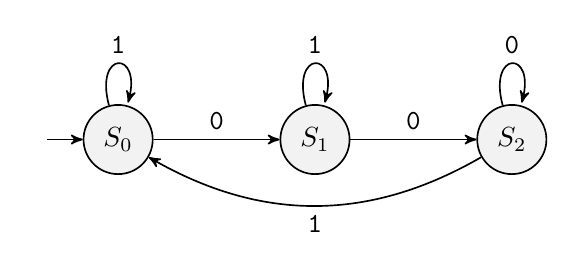
\begin{tikzpicture}
            \node[state, initial] (q1) {$S_0$};
            \node[state, right of=q1] (q2) {$S_1$};
            \node[state, right of=q2] (q3) {$S_2$};
            \draw (q1) edge[loop above] node {\tt 1} (q1);
            \draw (q1) edge node {\tt 0} (q2);
            \draw (q2) edge[loop above] node {\tt 1} (q2);
            \draw (q2) edge node {\tt 0} (q3);
            \draw (q3) edge[loop above] node {\tt 0} (q3);
            \draw (q3) edge[bend left] node {{\tt 1}} (q1);
            \end{tikzpicture}
    \end{center}
\end{figure}
We can represent this using a state table.
\begin{tabular}{c | c c | c}
    \toprule 
    Output state & Input = 0 & Input = 1 & Output \\
    \hline 
    $S_0$ & $S_1$ & $S_0$ & 0 \\
    $S_1$ & $S_2$ & $S_1$ & 1 \\
    $S_2$ & $S_2$ & $S_0$ & 0 \\
    \bottomrule
\end{tabular}

FSMs can be used as a \emph{recognizer}, a machine 
that outputs a 1 when the input string matches a 
certain description. Formally, there is one starting state. 
You feed it an input $\sigma$ which is a subset of 
all the possible strings you can create from the input alphabet. 
Then, the FSM outputs a 1 and we say it accepts the string. 
\end{document}
